% Standalone JAX training-stack slides (v5 companion to overview v4).
% Compile: latexmk -pdf slides-v5.tex  (from this directory)

\documentclass[11pt,aspectratio=43]{beamer}

\usepackage{amsmath,amssymb}
\usepackage{array,booktabs}
\usepackage{graphicx}
\usepackage{xcolor}
\graphicspath{{../v4/slides/}}
\usepackage{tikz}
\usetikzlibrary{arrows.meta,positioning,shapes.geometric,calc}

\definecolor{accent}{HTML}{2E75B6}
\definecolor{red2}{HTML}{C0392B}
\definecolor{green2}{HTML}{27AE60}
\definecolor{orange2}{HTML}{E67E22}

\setbeameroption{hide notes}
\setbeamertemplate{navigation symbols}{}
\setbeamersize{text margin left=0.9cm,text margin right=0.9cm}

\setbeamercolor{normal text}{fg=black,bg=white}
\setbeamercolor{frametitle}{fg=black,bg=white}
\setbeamercolor{title}{fg=black}
\setbeamercolor{structure}{fg=black}
\setbeamercolor{alerted text}{fg=accent}
\setbeamercolor{block title}{fg=black,bg=black!10}
\setbeamercolor{block body}{fg=black,bg=black!3}
\setbeamercolor{itemize item}{fg=black}
\setbeamercolor{itemize subitem}{fg=black}

\setbeamerfont{title}{size=\normalsize,series=\bfseries}
\setbeamerfont{frametitle}{size=\normalsize,series=\bfseries}
\setbeamerfont{block title}{size=\small,series=\bfseries}
\setbeamerfont{block body}{size=\small}

\setbeamertemplate{footline}{%
  \leavevmode%
  \hbox{%
    \begin{beamercolorbox}[wd=\paperwidth,ht=2.5ex,dp=1.0ex,rightskip=0.9cm]{author in head/foot}%
      \hfill\insertframenumber
    \end{beamercolorbox}%
  }%
}

\title{Octopus training stack:\\JAX side by side with SB3}
\author{Pulak Mehrotra}
\date{May 2026}

\begin{document}

\begin{frame}[plain]
  \titlepage
\end{frame}

\begin{frame}{The slow part is the simulator (CPU), not the neural net.}

\begin{columns}[T,onlytextwidth]
  \column{0.56\textwidth}
    \footnotesize
    \textbf{Realistic run} (reward~A, many traces, augmentation, \texttt{n\_envs=32})
    \vspace{0.3em}
    \begin{center}
      \begin{tabular}{@{}lr@{}}
        \toprule
        What we measure & Typical \\
        \midrule
        Time for 2M steps & $\approx$10.5 h \\
        Env steps per second & $\sim$50--56 \\
        GPU busy during train & $<10\%$ \\
        Long reset when cache misses & $\sim$120 ms \\
        \bottomrule
      \end{tabular}
    \end{center}
    \vspace{0.4em}
    \small Takeaway: time goes into \texttt{env.py} (reward, observations, bookkeeping) --- not PyTorch SAC.

  % Optional second column (napkin bar chart): uncomment \column + tikz + \end{columns} balance.
  % \column{0.42\textwidth} ...

\end{columns}

\end{frame}

% =========================================================================
% Policy outcome stays on SB3 (result they care about)
% =========================================================================

\begin{frame}{RL quality: SB3 stays the trusted path for results.}

\begin{columns}[T,onlytextwidth]
  \column{0.58\textwidth}
    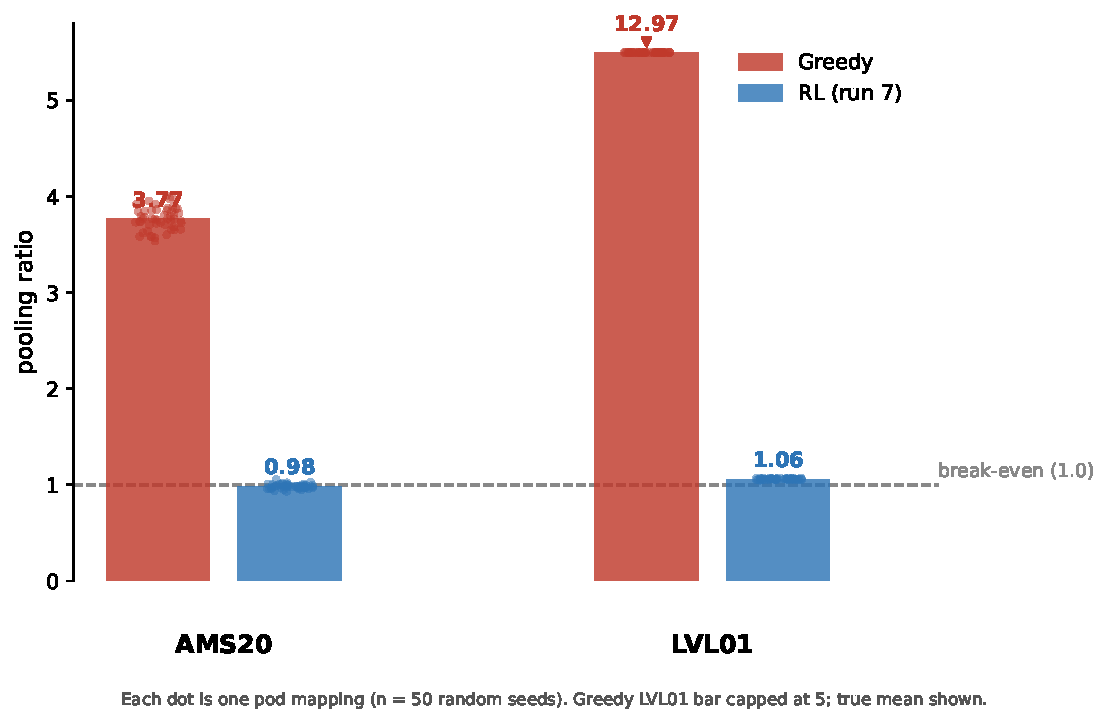
\includegraphics[width=\linewidth]{comparison_bar.pdf}
  \column{0.42\textwidth}
    \vspace{0.6em}
    \textbf{vs.\ baselines (pooling savings)}\\[0.4em]
    \small RL is the only rule that lands near break-even on \textbf{both}
    unseen traces; greedy does badly.
    \\[1em]
    \textbf{What JAX changes:}\\[0.2em]
    not the maths of the problem --- only \emph{how many steps per hour} we can run.
\end{columns}

\end{frame}

% =========================================================================
% SLIDE 1 / 5
% =========================================================================

\begin{frame}{Two ways to train: keep SB3, add JAX.}

  \vspace{0.3em}
  \begin{itemize}
    \setlength{\itemsep}{0.75em}
    \item \textbf{Baseline (trust this for papers):}\ \textbf{Gym + Stable-Baselines3 SAC} ---
          traces, augmentation, rewards, logging, offline eval hooks stay as today.
    \item \textbf{Parallel path (for speed):}\ \textbf{JAX} ---
          simulator state as plain arrays, \texttt{jit} stepping, bulk rollouts with \texttt{scan} and \texttt{vmap}.
    \item \textbf{Both see the same world:}\ same observations, same rewards (A/B/current), same episode setup --- so curves stay comparable.
    \item \textbf{Why JAX at all?}\ multiprocessing helps a lot, but Python still runs every env step.
          JAX pushes the stepping loop into compiled code so we can chew through timesteps cheaper.
  \end{itemize}

\end{frame}

% =========================================================================
% SLIDE 2 / 5
% =========================================================================

\begin{frame}[t]{Put the simulator in plain arrays (numpy now, JAX later).}

  \vspace{0.4em}
  \textbf{JAX packs the same numbers into one grouped object (\emph{pytree}):}\\[0.25em]
  \centering
  {\fontsize{9}{10}\selectfont\texttt{(mpd\_load,\; dealloc\_buf,\; host\_*\,,\; mpd\_dt/\allowbreak mpd\_mem/\allowbreak mpd\_n,\; rng\_key\,,\; indices)}}

  \vspace{0.35em}\raggedright
  {\scriptsize
  \emph{Concept:} one contiguous row per pool (numpy layout), grouped for \texttt{jit}.}
  {\scriptsize\setlength{\tabcolsep}{5pt}%
  \begin{tabular}{@{}r @{${}\Rightarrow{}$\ }p{\dimexpr\linewidth-3.4cm\relax}@{}}
    \toprule
    \multicolumn{1}{c}{\textbf{bank}} &
      \multicolumn{1}{l}{\textit{Packed row} (\texttt{\_mpd\_dt}, \texttt{\_mem}, \ldots)} \\
    \midrule
    0 & fixed slots \(\times\) VMs per pool \(\rightarrow\) scalar \texttt{\_mpd\_n[0]}\\
    \multicolumn{2}{l}{\(\vdots\) \ \(\ldots\) analogous rows \(\rightarrow\) \texttt{\_mpd\_n[1]}, \(\ldots\) \texttt{\_mpd\_n[}K$-1$\texttt{]}}\\
    \bottomrule
  \end{tabular}\par\vspace{0.08em}}
  {\fontsize{7}{8}\selectfont\color{black!53}%
  Not a nested list of Python tuples per alive VM --- arrays + counts.}

\end{frame}

% =========================================================================

\begin{frame}{Where Python stops and JAX starts each episode.}

\vspace{-0.2em}
\begingroup\footnotesize\centering
\textbf{Episode shape:}\ host builds tensors once,\ then GPU steps in a compiled loop.\par
\endgroup
\vspace{0.35em}

\centering
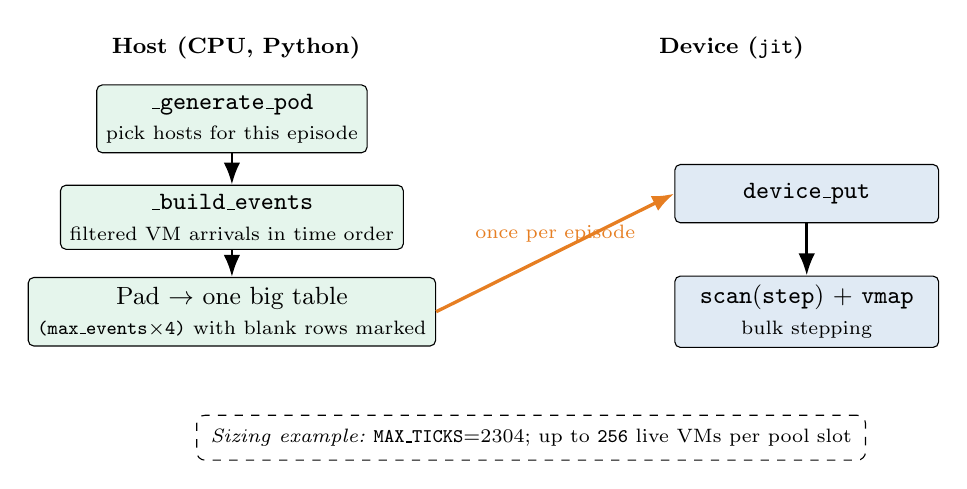
\begin{tikzpicture}[
    font=\small,
    host/.style={draw,rounded corners=2pt,fill=green2!12,minimum width=3.35cm,
                 minimum height=0.74cm,align=center},
    dev/.style={draw,rounded corners=2pt,fill=accent!15,minimum width=3.35cm,
                minimum height=0.74cm,align=center},
    arr/.style={-{Latex[length=2.8mm]},line width=1.0pt},
  ]
  \node[font=\footnotesize\bfseries,anchor=west] at (-5,-0.2) {Host (CPU, Python)};
  \node[host] (pod) at (-3.35, -1.1) {\texttt{\_generate\_pod}\\\scriptsize pick hosts for this episode};
  \node[host] (bld) at (-3.35, -2.35) {\texttt{\_build\_events}\\\scriptsize filtered VM arrivals in time order};
  \node[host] (pad) at (-3.35, -3.55)
    {Pad $\rightarrow$ one big table\\\scriptsize \texttt{(max\_events}$\times$\texttt{4)} with blank rows marked};
  \draw[arr] (pod) -- (bld);
  \draw[arr] (bld) -- (pad);

  \node[font=\footnotesize\bfseries,anchor=west] at (1.95,-0.2) {Device (\texttt{jit})};
  \node[dev] (dp) at (3.95, -2.05) {\texttt{device\_put}};
  \node[dev] (scan) at (3.95, -3.55) {\texttt{scan}(\texttt{step}) + \texttt{vmap}\\\scriptsize bulk stepping};
  \draw[arr,line width=1.2pt,orange2] (pad.east) -- node[above,font=\scriptsize]{once per episode} (dp.west);
  \draw[arr] (dp) -- (scan);

  \node[draw,dashed,rounded corners=3pt,inner sep=5pt,font=\scriptsize,align=left]
    at (0.45,-5.15)
    {\textit{Sizing example:}\ \texttt{MAX\_TICKS}=2304;\ up to \texttt{256}\ live VMs per pool slot};
\end{tikzpicture}

\end{frame}

% =========================================================================
% SLIDE 3 / 5
% =========================================================================

\begin{frame}[t,squeeze]{Same three stages; only the implementation changes.}

  \small
  Each numbered row means the same job on both sides.

  \vspace{0.25em}

  {\footnotesize
  \renewcommand{\arraystretch}{1.12}
  \setlength{\tabcolsep}{4pt}%
  \begin{tabular}{@{} >{\raggedright\arraybackslash}p{0.13\linewidth}
                  >{\raggedright\arraybackslash}p{0.365\linewidth}
                  >{\raggedright\arraybackslash}p{0.365\linewidth} @{}}
    \multicolumn{1}{c}{\textbf{Stage}} &
      \multicolumn{1}{c}{\textbf{SB3 + Gym + PyTorch}} &
      \multicolumn{1}{c}{\textbf{JAX + Optax (+ XLA)}} \\
    \midrule
    \textbf{1.}\newline Roll-out\newline \& gather &
      {\texttt{SubprocVecEnv} (\texttt{spawn}): numpy \texttt{OctopusMemPoolEnv.step()} per worker;\ observations to CUDA.\newline
       {\scriptsize\color{black!58}$\approx$\ same tuples}} &
      {\textbf{Compiled stepping:}\ \texttt{vmap} $\times$ \texttt{lax.scan}(\texttt{stepfn}). Arrays everywhere; RNG split per chunk;\ compiled inner loop.\newline
       {\scriptsize\color{black!58}no Python in the stepping hot path}} \\
    \addlinespace[0.15em]
    \midrule
    \textbf{2.}\newline Train\newline policy &
      {\textbf{SAC} (Stable-Baselines3): replay $\rightarrow$ \texttt{.learn()} minibatches $\rightarrow$ PyTorch on GPU.\newline
       {\scriptsize\color{black!58}same algorithm family}} &
      {\textbf{SAC} (ported): replay on CPU for now $\rightarrow$ one \texttt{jit} block for losses + optimizer;\newline
       {\scriptsize actor, twin critics, slow targets, auto~$\alpha$.}} \\
    \addlinespace[0.15em]
    \midrule
    \textbf{3.}\newline Log\newline \& test &
      {\textbf{Today:} TB/\,W\&B, checkpoints, eval callbacks; extra GPU worker scores pooling.\newline
       {\scriptsize\color{black!58}same dashboards / checkpoints}} &
      {\textbf{Todo:} checkpoints; Gym \& JAX episode parity tests; wire pooling scorer later.} \\
    \bottomrule
  \end{tabular}
  \par}

\end{frame}

% =========================================================================
% SLIDE 4 / 5
% =========================================================================

\begin{frame}{What gets compiled; what we want to measure.}

  \vspace{1em}
  \centering
  \footnotesize\textbf{Rough throughput picture}\\[0.35em]
  {\scriptsize
    Goal in speedup notes:\ finish 2M steps in \(\le\)3\,h \(\Rightarrow\) \(\sim\)185+ steps/s env-side.}
  \\[0.6em]

  {\footnotesize
    \renewcommand{\arraystretch}{1.15}
    \begin{tabular}{@{}>{\raggedright\arraybackslash}p{0.24\textwidth}
                    r
                    >{\raggedright\arraybackslash}p{0.58\textwidth}@{}}
      \toprule
      Situation & Rate & Comment \\
      \midrule
      Heavy config (meas.) & \(\sim\)53/s & reward~A etc.\\
      Sketch / light path & \(\sim\)1221/s & 32 workers, simpler inner loop\\
      Faster numpy env & TBD & vectorise + caches\\
      JAX full stack & TBD & full stack \& IO wired \\
      \bottomrule
    \end{tabular}
  \par}

\end{frame}

% =========================================================================
% SLIDE 5 / 5
% =========================================================================

% \begin{frame}{Takeaways}
%
%   \begin{itemize}
%     \setlength{\itemsep}{0.7em}
%     \item Papers and plots stay on the SB3 training path for now.
%     \item The roadmap spells what to wire up in order --- small tests guard the simulator.
%     \item JAX is about \textbf{hours per experiment}, not changing what ``good'' pooling means.
%     \item Other overview slides carry more RL-facing figures.
%   \end{itemize}
%
% \end{frame}

\end{document}
